\section{Arbejdsfordeling}
Projektet blev opdelt i to blokke: server og applikation. Da der blev valgt Xamarin som platform til applikationen og Firebase til serveren, skulle gruppen arbejde med nye tekonologier. Dette betød at der ikke var en den store erfaring, men plads til udvikling for gruppens medlemmer. \\
Ao arbejdede med serveropsætning, da han havde deltaget i nogle meet ups omkring Firebase og derfor havde en interesse for dette. Begge gruppe medlemmer fuldte en smartphone kursus på 6. semester, som der kunne drages lidt nytte af under udviklingen af applikationen. Der var dog også nyt stof, da det var en iOS applikation som skulle udvikles, hvor at kurset på 6. semester var i Android udvikling. \\
Selvom gruppens medlemmer havde forskellige ansvarsområder, blev alle vigtige beslutninger taget i fællesskab. Dette gjorde at hele gruppen havde et overordnet overblik over alle systemets dele.

For at holde overblik over arbejdsopgaverne, blev det brugt et scrum board. Dette værktøj kunne give et hurtigt indblik i hvad hvert enkelt gruppe medlem arbejdede med i øjeblikket. Boadet var også det centrale punkt i daglig scrum hver morgen, hvor man gennemgik hvad hver medlem arbejdede på i går og hvad man skulle videre med i dag. \\
På figur \ref{fig:Scrumboard} ses et billede af det overordnede fysiske scrum board.

\begin{figure} [H]
	\begin{center}
		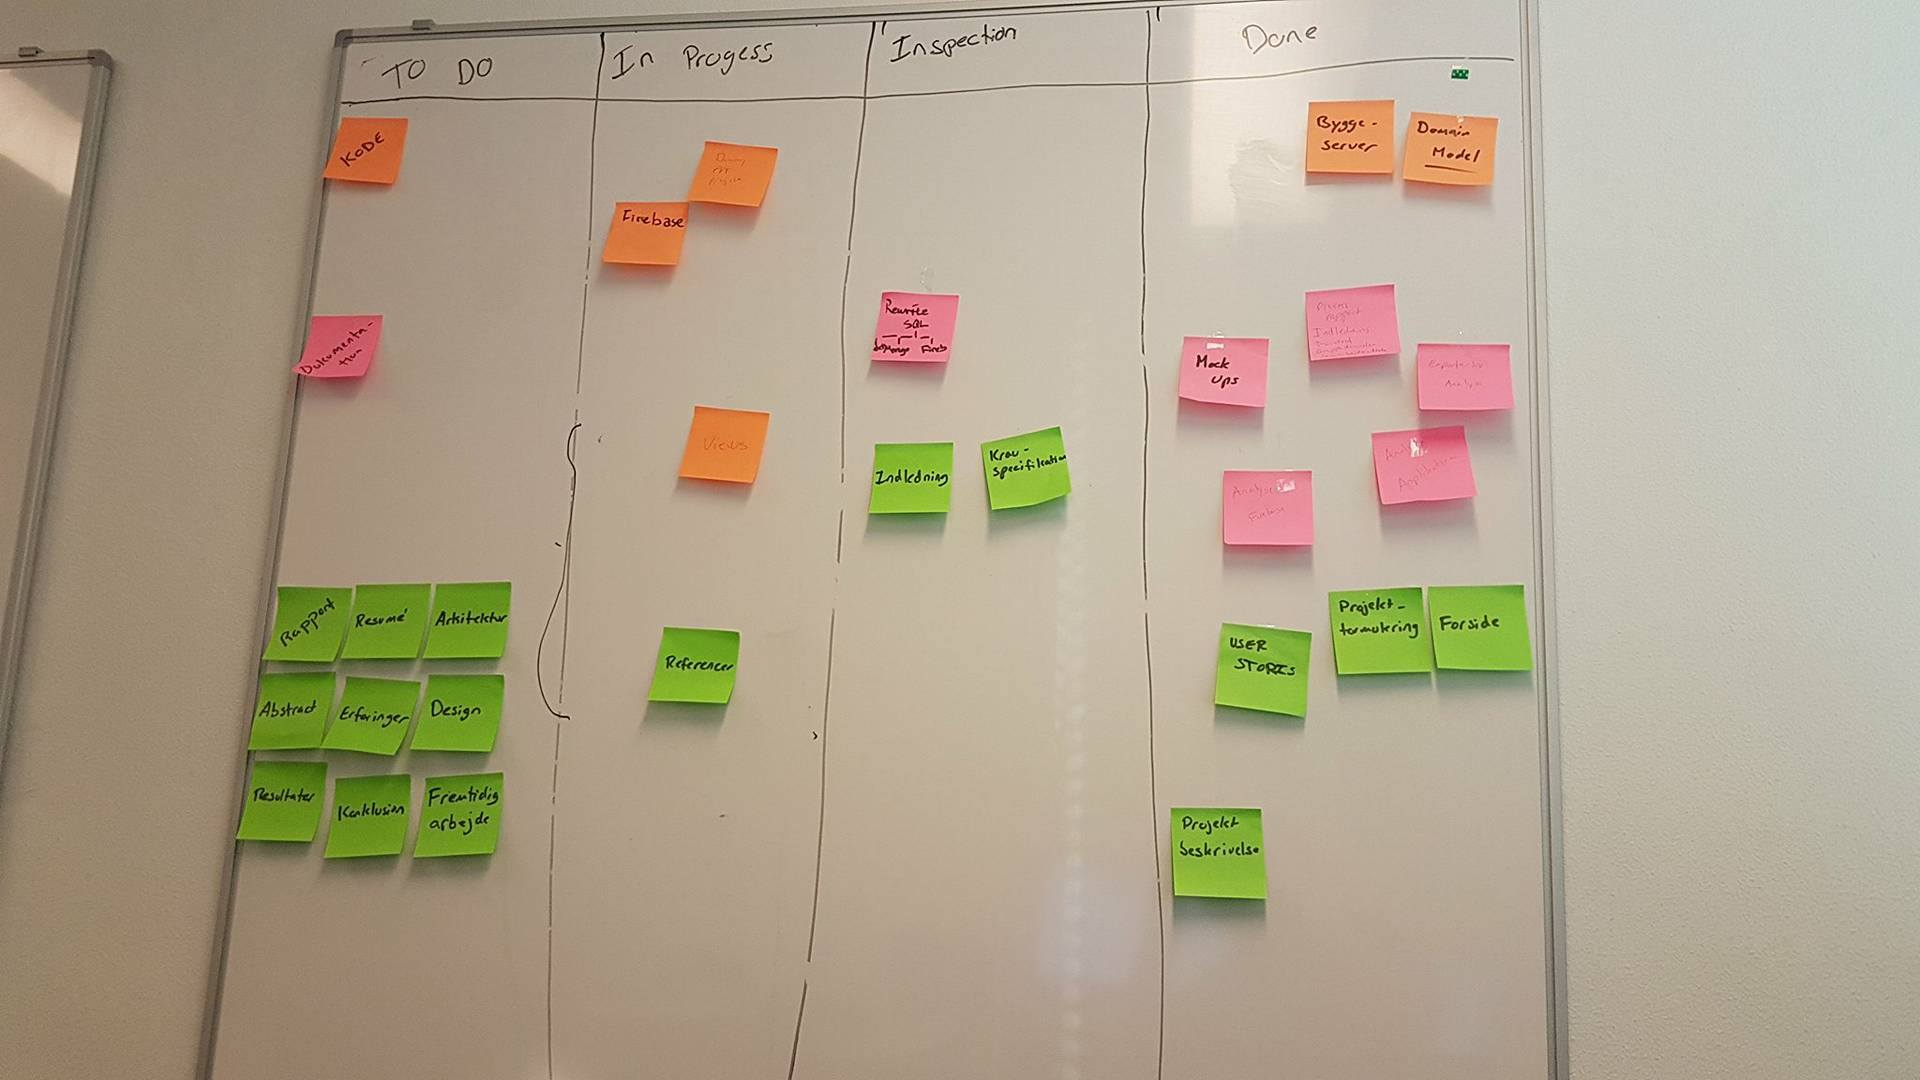
\includegraphics[height=8cm, width=12cm]{Arbejdsfordeling/ScrumBoard}
	\end{center}
	\caption{Scrum board}
	\label{fig:Scrumboard}
\end{figure}

For mere detaljeret scrum board, gå til bilag og se scrum screenshots. \\
Projektgruppen var tilfreds med arbejdsfordelingen. Opgavemængden var passende igennnem hele projektet. \\